\section{Our proposed solution}

We adopted POX, a Python-based controller,
as the basic controller for our work~\cite{pox}. It exports an
event-oriented interface, where the major events are the discovery of
switches and the reception of packets send by them to the
controller.
A module built on top of POX is a producer/consumer of events.
It can register
any event it creates with the \emph{core}, as well as subscribe to 
events registered by other modules.
To be able to handle different SDN protocols, POX encapsulates
all the details of the OpenFlow infrastructure inside an OpenFlow class
hierarchy.
On top of these basic events, POX constructs a set of
infrastructure modules that interact a publish/subscribe 
interface controlled by a \emph{core} element.

\subsection{POX original modules}

To implement the graph abstraction, we extended some of the modules already
available in POX to get the functionality we wanted. We first describe the
modules already available and their functionalities as provided by POX.
In the following sections we discuss how they were integrated and
how we created the
graph abstraction, with its associated interface.

The major module for our purposes is \texttt{Topology}. In the original POX
implementation, this module is responsible for maintaining the Network
Object Model (NOM), a dictionary of objects representing each \emph{entity}
(switch, router, host or other devices) in the network.
It
exports two 
methods, \emph{addEntity} and \emph{removeEntity}, which can be called by
other modules to register or delete entities that they are responsible for,
and
publishes two events, \emph{entityJoin} and \emph{entityLeave}, that may be
used by other modules that want to be notified of changes in the topology
of the network.

As mentioned previously, POX encapsulates all interaction with OpenFlow
elements in the OpenFlow class hierarchy (\texttt{of}).
The two major elements for our discussion are \texttt{of.discovery} and
\texttt{of.topology}. The first one implements the Link Layer Discovery
Protocol (LLDP), used to identify devices in the network~\cite{lldp}.
OpenFlow switches
should be able to identify other switches connected to them using this
protocol. The second module is responsible for interfacing with Topology to
store the identified entities (switches) in it.

Just as \emph{of.discovery} identifies switches, the \emph{host\_tracker}
module does the same for hosts. It does so by using a multitude of
techniques to identify and keep track of end hosts. The major element in
its operation is an ARP interceptor: all switches are programmed to send
\emph{ARPQuery} packets to the controller. If the query refers to a host
already known by the module, an \emph{ARPReply} message is built and sent
back to the host that initiated the query. At the same time, the location
of that host is recorded for future use. Periodically, \emph{host\_tracker}
issues fake \emph{ARPQuery} messages to every known host to verify if they
are still up. It may also access every switches counters to identify
activity on each link and infer host presence without issuing ARP messages.

Recently, POX received a DCHP module (\emph{misc.dhcpd})
that can be used to configure hosts in the
network. As available in the distribution, it has no interaction with the
topology system. However, the fact that it can be used to configure end
hosts provided an interesting opportunity in this work.

For our work, the modules just described, already present in POX,
had to be extended to build the
complete graph abstraction to represent a network. Those extensions are
described next.

\subsection{Changes needed for the new architecture}

Based on the functionalities of the existing modules,
we extended POX to build the graph abstraction. For that, the modules 
were extended to interact more closely with each other.
Figure~\ref{fig:design} shows the final architecture.

\begin{figure}[htb!]
    \centering
    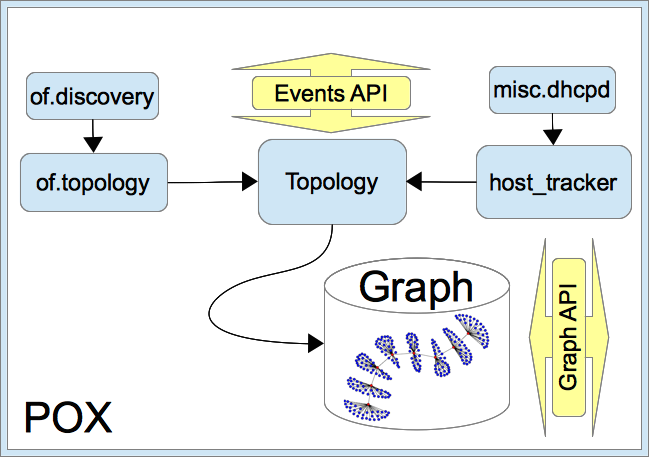
\includegraphics[width=0.9\columnwidth]{img/modules}
    \caption{Module integration}
    \label{fig:design}
\end{figure}

The \emph{entity} class was
extended through inheritance to hold all the information about each network
element, associated with the unique identifier already maintained by that
module.
The modules that discover and track network entities,
\emph{host\_tracker},
\emph{of.discovery}/\emph{of.topology}, and
\emph{misc.dhcpd},
create entities through \emph{topology}, which trigger events.
Those events are subscribed by the \emph{graph} module that creates, updates, 
deletes, executes algorithms and retrieves data from the network graph. 

\emph{Topology} was
extended to keep informations about links as entities, and to associate
events with them (like link up/down); \emph{of.discovery} keeps track of
links identified using LLDP, and \emph{of.topology} was altered to register
the links themselves with \emph{Topology}.

The new DCHP module (\emph{misc.dhcpd}) triggers \emph{DHCPLease} events
every time an IP address is associated with a host. \emph{Host\_tracker}
was extended to subscribe to that event. When notified, it updates its
active host database with that information, which helps in the process of
answering ARP queries (avoiding broadcasts) 

We altered \emph{host\_tracker} trigger events whenever a host is added or
removed.
\emph{Topology} listens to those events and
updates its object model accordingly, to keep track of all entities.
The event handler in this later module creates an instance of the
\emph{Host} class, which is added to the topology. The same behavior is
already used by \emph{of.topology} to add an instance of the \emph{Switch}
class to \emph{topology} when element of that kind is identified in the
network.

Similarly, when a switch stops responding to LLDP, a \emph{SwitchLeave}
event is triggered by \emph{of.topology}; when a host becomes inactive, 
does not answer to ARP probes sent by \emph{host\_tracker}, or generates no
observable traffic, a similar event is triggered. \emph{Topology}
listens to those events and updates its database.

\subsection{The graph abstraction and its module}

The proposed graph is represented by
$G=(V,E)$, in which $V$ and $E$ are finite sets of vertices and edges,
respectively.
Each vertex $v \in V$ represents one \emph{host} or  
\emph{switch} in the network. They are objects of class \emph{Entity} ---
to be precise, of its sub-classes \emph{Host} or \emph{Switch}.


Each edge $u \to v \in E$ represents a link between two vertices.
Edges between hosts and switches are derived indirectly through the events
of host addition or removal, assuming there is a link to the switch where
the host is first detected. It is essential, then, that
\emph{host\_tracker} notifies topology about the identity of the new host,
as well as the identifier for the switch and the port used. The system must
guarantee that such events are only generated by the switch to which the
host connects directly. That is achieved in our case because
no other packet can traverse the network from a host before
\emph{host\_tracker} identifies it (and its original switch) and adds
forwarding rules at that switch.
%
Edges between switches are identified by \emph{of.discovery} in the current
implementation. It publishes a \emph{LinkEvent} that notifies
\emph{of.topology} whether a link turns out to be \emph{up} or \emph{down}.
The later module updates the status of the associated switches. Originally,
that was not informed directly to \emph{topology}, though. In our solution,
a new kind of entity, \emph{Link}, was added, as well as the events
\emph{LinkJoin} and \emph{LinkLeave}, to fix that.

The edges weight $g(u, v)$ describes the traffic in bytes received and 
transmitted through the edge/\emph{link}.
The edge weight is obtained by periodically reading the counters from
the OpenFlow switches~\citep{openflow2013protocol}.
%The Table~\ref{table:counters} shows those counters.
%
%\begin{table}[htb!]
%    \centering
%    \begin{tabular}{| l | l |}
%    \hline
%    \textbf{Counters} & \textbf{Bits} \\ \hline
%    Received Packets & 64 \\ \hline
%    Transmitted Packets & 64 \\ \hline
%    Received Bytes & 64 \\ \hline
%    Transmitted Bytes & 64 \\ \hline
%    Received Drops & 64 \\ \hline
%    Transmitted Drops  & 64 \\ \hline
%    Received Errors & 64 \\ \hline
%    Transmitted Errors & 64 \\ \hline
%    Received Frame Errors & 64 \\ \hline
%    Transmitted Overflow errors & 64 \\ \hline
%    Received CRC Errors & 64 \\ \hline
%    Collisions & 64 \\
%    \hline
%    \end{tabular}
%    \caption{Port Counters by Port}
%    \label{table:counters}
%\end{table}

On its
turn, every time \emph{topology} identifies a change in the network, it
triggers a related event, \emph{topologyUpdate}, so that
other modules that may want to keep track of that can do so. The Graph
module will do just that, and react to any changes triggered by any
publisher in one of the channels observed by \emph{topology}.


\subsection{Programming Interface (API)}

The graph module has an application programming interface (API) so that
other modules of the controller can retrieve information about the network
topology from it.

\begin{outline}
\0 The major graph methods are:
    \1 \emph{get\_vertex(id)}:
    Returns an entity of the graph (\emph{host}/\emph{switch}).
    \1 \emph{get\_adjacents(id)}: 
    Returns the adjacency list of a vertex.
    \1 \emph{snapshot()}: 
    Copy the graph in the form of two collections (vertices and edges)
    \1 \emph{to\_dot(harq, layout = "dot")}:
    Create a copy of the graph to be used by Graphviz~\citep{john2003graphviz}.
%\0 Os Algoritmos de grafos já implementados são:
%    \1 \emph{get\_mst()}:
%    Return the minimum spanning tree of the graph in real time.
\end{outline}

Besides that,
the module is fully extensible, and our goal is that different graph
algorithms may be implemented by developers or the end users, and always
retrofitted to the module, so they can become available to others. By doing
so, code reuse is maximized; anyone implementing a different
version of a routing algorithm could benefit from a previously implemented
shortest path algorithm, for example. Right now, just a minimum spanning
tree algorithm has been implemented, being available through the method
\emph{get\_mst()}.
